% Generated by code/needham.py -- do not edit by hand.
\definecolor{qocA}{rgb}{0.00,0.45,0.70}
\definecolor{qocB}{rgb}{0.90,0.60,0.00}
\definecolor{qocC}{rgb}{0.00,0.62,0.45}
\definecolor{qocD}{rgb}{0.80,0.40,0.00}
\definecolor{qocE}{rgb}{0.80,0.60,0.70}
\definecolor{qocF}{rgb}{0.35,0.70,0.90}
\begin{tikzpicture}[ink/.style={line width=0.9pt, ndInk}, faint/.style={line width=0.4pt, ndInk!35}, dashedink/.style={line width=0.5pt, ndInk!55, dash pattern=on 2.5pt off 2pt}, vec/.style={->, >=stealth, line width=1.2pt}, note/.style={font=\footnotesize\itshape, text=ndInk!85, align=center}, pointer/.style={->, >=stealth, line width=0.4pt, ndInk!60, shorten >=2pt, shorten <=1pt}, dot/.style={circle, fill=ndInk, inner sep=0pt, minimum size=3.4pt}, wash/.style={fill=ndSky, fill opacity=0.55}, every node/.style={text=ndInk}]
\definecolor{ndInk}{rgb}{0.13,0.13,0.18}
\definecolor{ndPaper}{rgb}{0.99,0.96,0.88}
\definecolor{ndSky}{rgb}{0.84,0.91,0.98}
\definecolor{ndRose}{rgb}{0.98,0.86,0.84}
\definecolor{ndBlue}{rgb}{0.13,0.36,0.66}
\definecolor{ndRed}{rgb}{0.78,0.20,0.16}
\definecolor{ndGold}{rgb}{0.88,0.62,0.10}
\definecolor{ndGreen}{rgb}{0.18,0.52,0.30}
\fill[ndSky, fill opacity=0.7, rounded corners=9pt] (0.95,5.43) rectangle (3.00,7.47);
\fill[ndGold!30, fill opacity=0.7, rounded corners=9pt] (2.05,5.37) rectangle (5.80,7.53);
\fill[ndSky, fill opacity=0.7, rounded corners=9pt] (4.85,5.43) rectangle (8.60,7.47);
\fill[ndGold!30, fill opacity=0.7, rounded corners=9pt] (10.25,5.37) rectangle (12.80,7.53);
\fill[ndSky, fill opacity=0.7, rounded corners=9pt] (11.85,5.43) rectangle (15.60,7.47);
\node[draw=ndInk, fill=white, circle, inner sep=1.2pt, minimum size=0.62cm, font=\small] (x0) at (1.40,5.85) {$x_{1}$};
\node[draw=ndBlue, line width=0.9pt, fill=white, rounded corners=3pt, inner sep=2pt, minimum height=0.6cm, font=\small] (s0) at (2.50,7.05) {$s_{1}$};
\node[draw=ndInk, fill=white, circle, inner sep=1.2pt, minimum size=0.62cm, font=\small] (x1) at (4.20,5.85) {$x_{2}$};
\node[draw=ndBlue, line width=0.9pt, fill=white, rounded corners=3pt, inner sep=2pt, minimum height=0.6cm, font=\small] (s1) at (5.30,7.05) {$s_{2}$};
\node[draw=ndInk, fill=white, circle, inner sep=1.2pt, minimum size=0.62cm, font=\small] (x2) at (7.00,5.85) {$x_{3}$};
\node[draw=ndBlue, line width=0.9pt, fill=white, rounded corners=3pt, inner sep=2pt, minimum height=0.6cm, font=\small] (s2) at (8.10,7.05) {$s_{3}$};
\node[draw=ndInk, fill=white, circle, inner sep=1.2pt, minimum size=0.62cm, font=\small] (x3) at (11.20,5.85) {$x_{n-1}$};
\node[draw=ndBlue, line width=0.9pt, fill=white, rounded corners=3pt, inner sep=2pt, minimum height=0.6cm, font=\small] (s3) at (12.30,7.05) {$s_{n-1}$};
\node[draw=ndInk, fill=white, circle, inner sep=1.2pt, minimum size=0.62cm, font=\small] (x4) at (14.00,5.85) {$x_{n}$};
\node[draw=ndRed, line width=0.9pt, fill=white, rounded corners=3pt, inner sep=2pt, minimum height=0.6cm, font=\small] (p) at (15.10,7.05) {$p_n$};
\draw[->, >=stealth, line width=0.6pt, ndInk!70] (x0) -- (s0);
\draw[->, >=stealth, line width=0.6pt, ndInk!70] (x1) -- (s1);
\draw[->, >=stealth, line width=0.9pt, ndBlue] (s0) -- (s1);
\draw[->, >=stealth, line width=0.6pt, ndInk!70] (x2) -- (s2);
\draw[->, >=stealth, line width=0.9pt, ndBlue] (s1) -- (s2);
\draw[->, >=stealth, line width=0.6pt, ndInk!70] (x3) -- (s3);
\draw[->, >=stealth, line width=0.6pt, ndInk!70, dash pattern=on 2pt off 2pt] (s1) -- (s2.west);
\node[font=\small] at (9.65,7.05) {$\cdots$};
\draw[->, >=stealth, line width=0.6pt, ndInk!70] (x4) -- (p);
\draw[->, >=stealth, line width=0.9pt, ndBlue] (s3) -- (p);
\node[note, anchor=west] at (1.00,7.90) {$s_k=F(s_{k-1},x_k)$: the populations $(p_k,1-p_k)$ after the step $k$};
\node[note, anchor=north] at (8.20,5.30) {each wash is one clique $\{s_{k-1},x_k,s_k\}$ of five variables: one PSD block of order $21$, whatever $n$};
\node[font=\small, anchor=north] at (8.20,4.80) {(a) the record as a chain, with its states lifted to variables};
\draw[faint, ->, >=stealth] (0.600,0.000) -- (5.072,0.000) node[right, text=ndInk] {{\scriptsize $n$}};
\draw[faint, ->, >=stealth] (0.600,0.000) -- (0.600,3.392) node[above, text=ndInk] {{\scriptsize population after $n$ steps}};
\draw[faint] (0.949,0.060) -- (0.949,-0.060) node[below, font=\scriptsize, text=ndInk] {$4$};
\draw[faint] (2.343,0.060) -- (2.343,-0.060) node[below, font=\scriptsize, text=ndInk] {$10$};
\draw[faint] (4.668,0.060) -- (4.668,-0.060) node[below, font=\scriptsize, text=ndInk] {$20$};
\draw[faint] (0.660,1.600) -- (0.540,1.600) node[left, font=\scriptsize, text=ndInk] {$\tfrac12$};
\draw[faint] (0.660,3.200) -- (0.540,3.200) node[left, font=\scriptsize, text=ndInk] {$1$};
\fill[ndSky, fill opacity=0.6] (0.716,2.766) -- (0.949,2.650) -- (1.181,2.545) -- (1.414,2.450) -- (1.646,2.365) -- (1.878,2.289) -- (2.111,2.220) -- (2.343,2.158) -- (2.576,2.102) -- (2.808,2.052) -- (3.041,2.007) -- (3.273,1.966) -- (3.505,1.929) -- (3.738,1.896) -- (3.970,1.867) -- (4.203,1.840) -- (4.435,1.816) -- (4.668,1.795) -- (4.668,0.010) -- (4.435,0.014) -- (4.203,0.018) -- (3.970,0.024) -- (3.738,0.032) -- (3.505,0.043) -- (3.273,0.057) -- (3.041,0.076) -- (2.808,0.101) -- (2.576,0.135) -- (2.343,0.180) -- (2.111,0.240) -- (1.878,0.320) -- (1.646,0.427) -- (1.414,0.570) -- (1.181,0.759) -- (0.949,1.012) -- (0.716,1.350) -- cycle;
\draw[line width=0.9pt, ndInk] (0.716,2.766) -- (0.949,2.650) -- (1.181,2.545) -- (1.414,2.450) -- (1.646,2.365) -- (1.878,2.289) -- (2.111,2.220) -- (2.343,2.158) -- (2.576,2.102) -- (2.808,2.052) -- (3.041,2.007) -- (3.273,1.966) -- (3.505,1.929) -- (3.738,1.896) -- (3.970,1.867) -- (4.203,1.840) -- (4.435,1.816) -- (4.668,1.795);
\draw[line width=0.9pt, ndInk, dash pattern=on 3pt off 2pt] (0.716,1.350) -- (0.949,1.012) -- (1.181,0.759) -- (1.414,0.570) -- (1.646,0.427) -- (1.878,0.320) -- (2.111,0.240) -- (2.343,0.180) -- (2.576,0.135) -- (2.808,0.101) -- (3.041,0.076) -- (3.273,0.057) -- (3.505,0.043) -- (3.738,0.032) -- (3.970,0.024) -- (4.203,0.018) -- (4.435,0.014) -- (4.668,0.010);
\draw[ndRed, line width=0.8pt] (0.889,2.590) -- (1.009,2.710) (0.889,2.710) -- (1.009,2.590);
\draw[ndRed, line width=0.8pt] (1.354,2.398) -- (1.474,2.518) (1.354,2.518) -- (1.474,2.398);
\draw[ndRed, line width=0.8pt] (2.283,2.509) -- (2.403,2.629) (2.283,2.629) -- (2.403,2.509);
\draw[ndRed, line width=0.8pt] (2.748,3.045) -- (2.868,3.165) (2.748,3.165) -- (2.868,3.045);
\draw[->, >=stealth, ndRed, line width=0.6pt] (3.738,3.080) -- (3.738,3.320) node[above, font=\tiny, text=ndRed] {1.9};
\draw[->, >=stealth, ndRed, line width=0.6pt] (4.668,3.080) -- (4.668,3.320) node[above, font=\tiny, text=ndRed] {4.2};
\draw[ndRed, line width=0.7pt, fill=white] (1.878,1.551) circle (1.8pt);
\draw[ndBlue, line width=0.7pt, fill=white] (0.894,2.595) rectangle (1.004,2.705);
\draw[ndBlue, line width=0.7pt, fill=white] (1.359,2.395) rectangle (1.469,2.505);
\draw[ndBlue, line width=0.7pt, fill=white] (1.823,2.234) rectangle (1.933,2.344);
\draw[ndBlue, line width=0.7pt, fill=white] (2.288,2.103) rectangle (2.398,2.213);
\draw[ndBlue, line width=0.7pt, fill=white] (2.753,1.997) rectangle (2.863,2.107);
\draw[ndBlue, line width=0.7pt, fill=white] (3.683,1.841) rectangle (3.793,1.951);
\fill[ndBlue] (0.949,2.650) circle (1.6pt);
\fill[ndBlue] (1.414,2.450) circle (1.6pt);
\fill[ndBlue] (1.878,2.289) circle (1.6pt);
\fill[ndBlue] (2.343,2.158) circle (1.6pt);
\fill[ndBlue] (2.808,2.052) circle (1.6pt);
\fill[ndBlue] (3.738,1.896) circle (1.6pt);
\fill[ndBlue] (4.668,1.795) circle (1.6pt);
\fill[ndGreen] (0.949,1.012) circle (1.6pt);
\fill[ndGreen] (1.414,0.570) circle (1.6pt);
\fill[ndGreen] (1.878,0.320) circle (1.6pt);
\fill[ndGreen] (2.343,0.180) circle (1.6pt);
\fill[ndGreen] (2.808,0.101) circle (1.6pt);
\node[note, anchor=south west] at (0.716,2.816) {$\frac12+\frac12\,0.9^n$};
\node[note, anchor=south west] at (1.088,1.024) {$0.75^n$};
\fill[ndBlue] (2.622,1.568) circle (1.6pt);
\node[font=\tiny, anchor=west, text=ndInk] at (2.762,1.568) {upper, SL-chord 2};
\draw[ndBlue, line width=0.7pt, fill=white] (2.567,1.273) rectangle (2.677,1.383);
\node[font=\tiny, anchor=west, text=ndInk] at (2.762,1.328) {upper, SL-push 3};
\draw[ndRed, line width=0.8pt] (2.562,1.028) -- (2.682,1.148) (2.562,1.148) -- (2.682,1.028);
\node[font=\tiny, anchor=west, text=ndInk] at (2.762,1.088) {upper, SL-push 2};
\fill[ndGreen] (2.622,0.848) circle (1.6pt);
\node[font=\tiny, anchor=west, text=ndInk] at (2.762,0.848) {lower, SL-push 3};
\draw[ndRed, line width=0.7pt, fill=white] (2.622,0.608) circle (1.8pt);
\node[font=\tiny, anchor=north west, text=ndInk, align=left] at (2.762,0.720) {SL-push 2 at $n=8$: SCS\\ inaccurate, not a bound};
\node[font=\small, anchor=north] at (2.750,-0.768) {(b) the certified band};
\draw[faint, ->, >=stealth] (6.300,0.000) -- (10.772,0.000) node[right, text=ndInk] {{\scriptsize $n$}};
\draw[faint, ->, >=stealth] (6.300,0.000) -- (6.300,3.392) node[above, text=ndInk] {{\scriptsize order of the largest PSD block}};
\draw[faint] (6.649,0.060) -- (6.649,-0.060) node[below, font=\scriptsize, text=ndInk] {$4$};
\draw[faint] (8.043,0.060) -- (8.043,-0.060) node[below, font=\scriptsize, text=ndInk] {$10$};
\draw[faint] (10.368,0.060) -- (10.368,-0.060) node[below, font=\scriptsize, text=ndInk] {$20$};
\draw[faint] (6.360,0.267) -- (6.240,0.267) node[left, font=\scriptsize, text=ndInk] {$10$};
\draw[faint] (6.360,1.067) -- (6.240,1.067) node[left, font=\scriptsize, text=ndInk] {$10^4$};
\draw[faint] (6.360,2.133) -- (6.240,2.133) node[left, font=\scriptsize, text=ndInk] {$10^8$};
\draw[faint] (6.360,3.200) -- (6.240,3.200) node[left, font=\scriptsize, text=ndInk] {$10^{12}$};
\draw[line width=0.9pt, ndInk, dash pattern=on 3pt off 2pt] (6.416,0.347) -- (6.649,0.492) -- (6.881,0.640) -- (7.114,0.791) -- (7.346,0.943) -- (7.578,1.096) -- (7.811,1.250) -- (8.043,1.404) -- (8.276,1.560) -- (8.508,1.715) -- (8.741,1.871) -- (8.973,2.028) -- (9.205,2.184) -- (9.438,2.341) -- (9.670,2.498) -- (9.903,2.655) -- (10.135,2.813) -- (10.368,2.971);
\fill[ndInk] (6.416,0.347) circle (1.6pt);
\fill[ndInk] (6.649,0.492) circle (1.6pt);
\draw[line width=0.9pt, ndBlue] (6.416,0.353) -- (10.368,0.353);
\draw[line width=0.9pt, ndBlue!55] (6.416,0.347) -- (10.368,0.347);
\draw[line width=0.9pt, ndRed] (6.416,0.267) -- (10.368,0.267);
\node[font=\tiny, anchor=south east, text=ndBlue] at (10.554,0.379) {SL-chord $21$, SL-push 3 $20$};
\node[font=\tiny, anchor=north east, text=ndRed] at (10.554,0.245) {SL-push 2 $10$};
\node[note, anchor=south west] at (8.624,0.640) {lifted:\\ constant in $n$};
\node[note, anchor=west] at (6.556,2.560) {dense: $\binom{2n}{n}$,\\ $1.4\cdot10^{11}$ at $n=20$};
\node[font=\small, anchor=north] at (8.450,-0.533) {(c) the size of the SDP};
\draw[faint, ->, >=stealth] (12.000,0.000) -- (16.472,0.000) node[right, text=ndInk] {{\scriptsize $n$}};
\draw[faint, ->, >=stealth] (12.000,0.000) -- (12.000,3.392) node[above, text=ndInk] {{\scriptsize seconds (SCS)}};
\draw[faint] (12.349,0.060) -- (12.349,-0.060) node[below, font=\scriptsize, text=ndInk] {$4$};
\draw[faint] (13.743,0.060) -- (13.743,-0.060) node[below, font=\scriptsize, text=ndInk] {$10$};
\draw[faint] (16.068,0.060) -- (16.068,-0.060) node[below, font=\scriptsize, text=ndInk] {$20$};
\draw[faint] (12.060,0.000) -- (11.940,0.000) node[left, font=\scriptsize, text=ndInk] {$0.1$};
\draw[faint] (12.060,0.914) -- (11.940,0.914) node[left, font=\scriptsize, text=ndInk] {$1$};
\draw[faint] (12.060,1.829) -- (11.940,1.829) node[left, font=\scriptsize, text=ndInk] {$10$};
\draw[faint] (12.060,2.743) -- (11.940,2.743) node[left, font=\scriptsize, text=ndInk] {$100$};
\draw[line width=0.6pt, ndBlue] (12.349,0.845) -- (12.814,1.211) -- (13.278,1.499) -- (13.743,1.530) -- (14.208,1.786) -- (15.138,2.139) -- (16.068,2.472);
\fill[ndBlue] (12.349,0.845) circle (1.6pt);
\fill[ndBlue] (12.814,1.211) circle (1.6pt);
\fill[ndBlue] (13.278,1.499) circle (1.6pt);
\fill[ndBlue] (13.743,1.530) circle (1.6pt);
\fill[ndBlue] (14.208,1.786) circle (1.6pt);
\fill[ndBlue] (15.138,2.139) circle (1.6pt);
\fill[ndBlue] (16.068,2.472) circle (1.6pt);
\draw[line width=0.6pt, ndBlue] (12.349,0.994) -- (12.814,1.171) -- (13.278,1.455) -- (13.743,1.568) -- (14.208,1.614) -- (15.138,1.962);
\draw[ndBlue, line width=0.7pt, fill=white] (12.294,0.939) rectangle (12.404,1.049);
\draw[ndBlue, line width=0.7pt, fill=white] (12.759,1.116) rectangle (12.869,1.226);
\draw[ndBlue, line width=0.7pt, fill=white] (13.223,1.400) rectangle (13.333,1.510);
\draw[ndBlue, line width=0.7pt, fill=white] (13.688,1.513) rectangle (13.798,1.623);
\draw[ndBlue, line width=0.7pt, fill=white] (14.153,1.559) rectangle (14.263,1.669);
\draw[ndBlue, line width=0.7pt, fill=white] (15.083,1.907) rectangle (15.193,2.017);
\draw[line width=0.6pt, ndRed] (12.349,1.085) -- (12.814,1.183) -- (13.743,1.375) -- (14.208,1.273) -- (15.138,1.419) -- (16.068,1.804);
\draw[ndRed, line width=0.8pt] (12.289,1.025) -- (12.409,1.145) (12.289,1.145) -- (12.409,1.025);
\draw[ndRed, line width=0.8pt] (12.754,1.123) -- (12.874,1.243) (12.754,1.243) -- (12.874,1.123);
\draw[ndRed, line width=0.8pt] (13.683,1.315) -- (13.803,1.435) (13.683,1.435) -- (13.803,1.315);
\draw[ndRed, line width=0.8pt] (14.148,1.213) -- (14.268,1.333) (14.148,1.333) -- (14.268,1.213);
\draw[ndRed, line width=0.8pt] (15.078,1.359) -- (15.198,1.479) (15.078,1.479) -- (15.198,1.359);
\draw[ndRed, line width=0.8pt] (16.008,1.744) -- (16.128,1.864) (16.008,1.864) -- (16.128,1.744);
\draw[line width=0.9pt, ndInk, dash pattern=on 3pt off 2pt] (12.116,0.276) -- (12.349,1.604);
\fill[ndInk] (12.116,0.276) circle (1.6pt);
\fill[ndInk] (12.349,1.604) circle (1.6pt);
\node[note, anchor=north west] at (12.163,3.154) {dense, solved\\ for $n=3,4$ only};
\node[note, anchor=east, text=ndBlue] (tc) at (15.975,1.051) {SL-chord at\\ $n=20$: 51 s};
\draw[pointer] (tc.east) to[bend right=20] (16.068,2.381);
\fill[ndBlue] (12.628,0.640) circle (1.6pt);
\node[font=\tiny, anchor=west, text=ndInk] at (12.767,0.640) {SL-chord, order 2};
\draw[ndBlue, line width=0.7pt, fill=white] (12.573,0.402) rectangle (12.683,0.512);
\node[font=\tiny, anchor=west, text=ndInk] at (12.767,0.457) {SL-push, order 3};
\draw[ndRed, line width=0.8pt] (12.568,0.214) -- (12.688,0.334) (12.568,0.334) -- (12.688,0.214);
\node[font=\tiny, anchor=west, text=ndInk] at (12.767,0.274) {SL-push, order 2};
\fill[ndInk] (12.628,0.091) circle (1.6pt);
\node[font=\tiny, anchor=west, text=ndInk] at (12.767,0.091) {dense};
\node[font=\small, anchor=north] at (14.150,-0.594) {(d) the solve times};
\end{tikzpicture}
